\documentclass[letterpaper, 12pt]{article}
\usepackage{mathtools}
\DeclarePairedDelimiter\abs{\lvert}{\rvert}     %serve per mettere il modulo 
\usepackage{booktabs}
\usepackage{bm}
\usepackage{textcomp}
\usepackage{colortbl}
\usepackage{tabularx}
\usepackage{siunitx}
\usepackage{enumitem}
\usepackage{xcolor}
\usepackage{fancyhdr}
\usepackage{caption}
\usepackage{changepage}
\usepackage{amsmath} 
\usepackage{subcaption}
\usepackage{graphicx}
\usepackage[table]{xcolor} 
\usepackage[margin=1in,letterpaper]{geometry} % decreases margins
\usepackage{cite} % takes care of citations
\usepackage[hidelinks]{hyperref} % adds hyper links inside the generated pdf file
\usepackage{blindtext}

% Setup hyperref
\hypersetup{
    colorlinks=false, % colored links
    linkcolor=linkcolor, % color for internal links
    citecolor=citecolor, % color for citations
    urlcolor=urlcolor, % color for URLs
}
\fancypagestyle{logoheader}{
    \fancyhf{}
    \fancyhead[L]{
\includegraphics[width = 3cm]{logo_bicocca.png}}
    \renewcommand{\headrulewidth}{0pt}
}
\setlength{\headheight}{72.63475pt} % Fix fancyhdr warning
\addtolength{\topmargin}{-0.75pt} % Compensate for increased headheight

\graphicspath{{immagini/}}
%Required for inserting images
%++++++++++++++++++++++++++++++++++++++++
%Margini 


\begin{document}


\title{{\small Università degli studi Milano Bicocca - Dipartimento di Fisica}\\
	Esperimentazioni di Fisica Computazionale}
\author{S. Franceschina}
\date{\today}
\maketitle
\thispagestyle{logoheader}

%Abstract da completare
\begin{abstract} 
	\begin{adjustwidth}{-1cm}{-1cm}
	\end{adjustwidth}
\end{abstract}
\tableofcontents
\newpage

\section{Analisi dell'errore}
\subsection{Teoria}
Nella presente sezione analizziamo le due principali fonti di errore in contesti computazionali: 
\begin{enumerate}
    \item Errori di arrotondamento: dovuti alla rappresentazione di numeri reali con numero finito di digits.
    \item Errori di approssimazione: dovuti alla modalità stessa con cui affrontiamo il problema, 
          per questo motivo sono presenti anche nel caso ideale. 
\end{enumerate}

\subsection{Esercizio 1.0.1}
Considera la funzione $f(x)=e^x$ nell'intervallo $x\in [0,1]$. Scrivi un programma che calcoli la serie approssimante:

$$
    g_N(x)=\sum_{n=0}^N \frac{x^n}{n!}\,.
$$

\begin{enumerate}
    \item Verifica che l'errore assoluto $\Delta=|f(x)-g_N(x)|$ scala approssimativamente come $x^{N+1}/(N+1)!$ per $N=1,2,3,4$.
    \item L'errore $\Delta$, nell'intervallo dato di $x$, differisce da $x^{N+1}/(N+1)!$. Perché accade questo e per quali valori di $x$?
\end{enumerate}

\subsubsection{Soluzione}
Al fine dell'esercizio vengono rappresentati nel grafico \ref{fig:es1_0_1_1} le funzioni $\Delta$ e $\frac{x^{N+1}}{(N+1)!}$, con 
$N=1,2,3, 4$, al variare di $x$ nell'intervallo $[0,1]$. 

\begin{figure}[ht!]
    \centering
    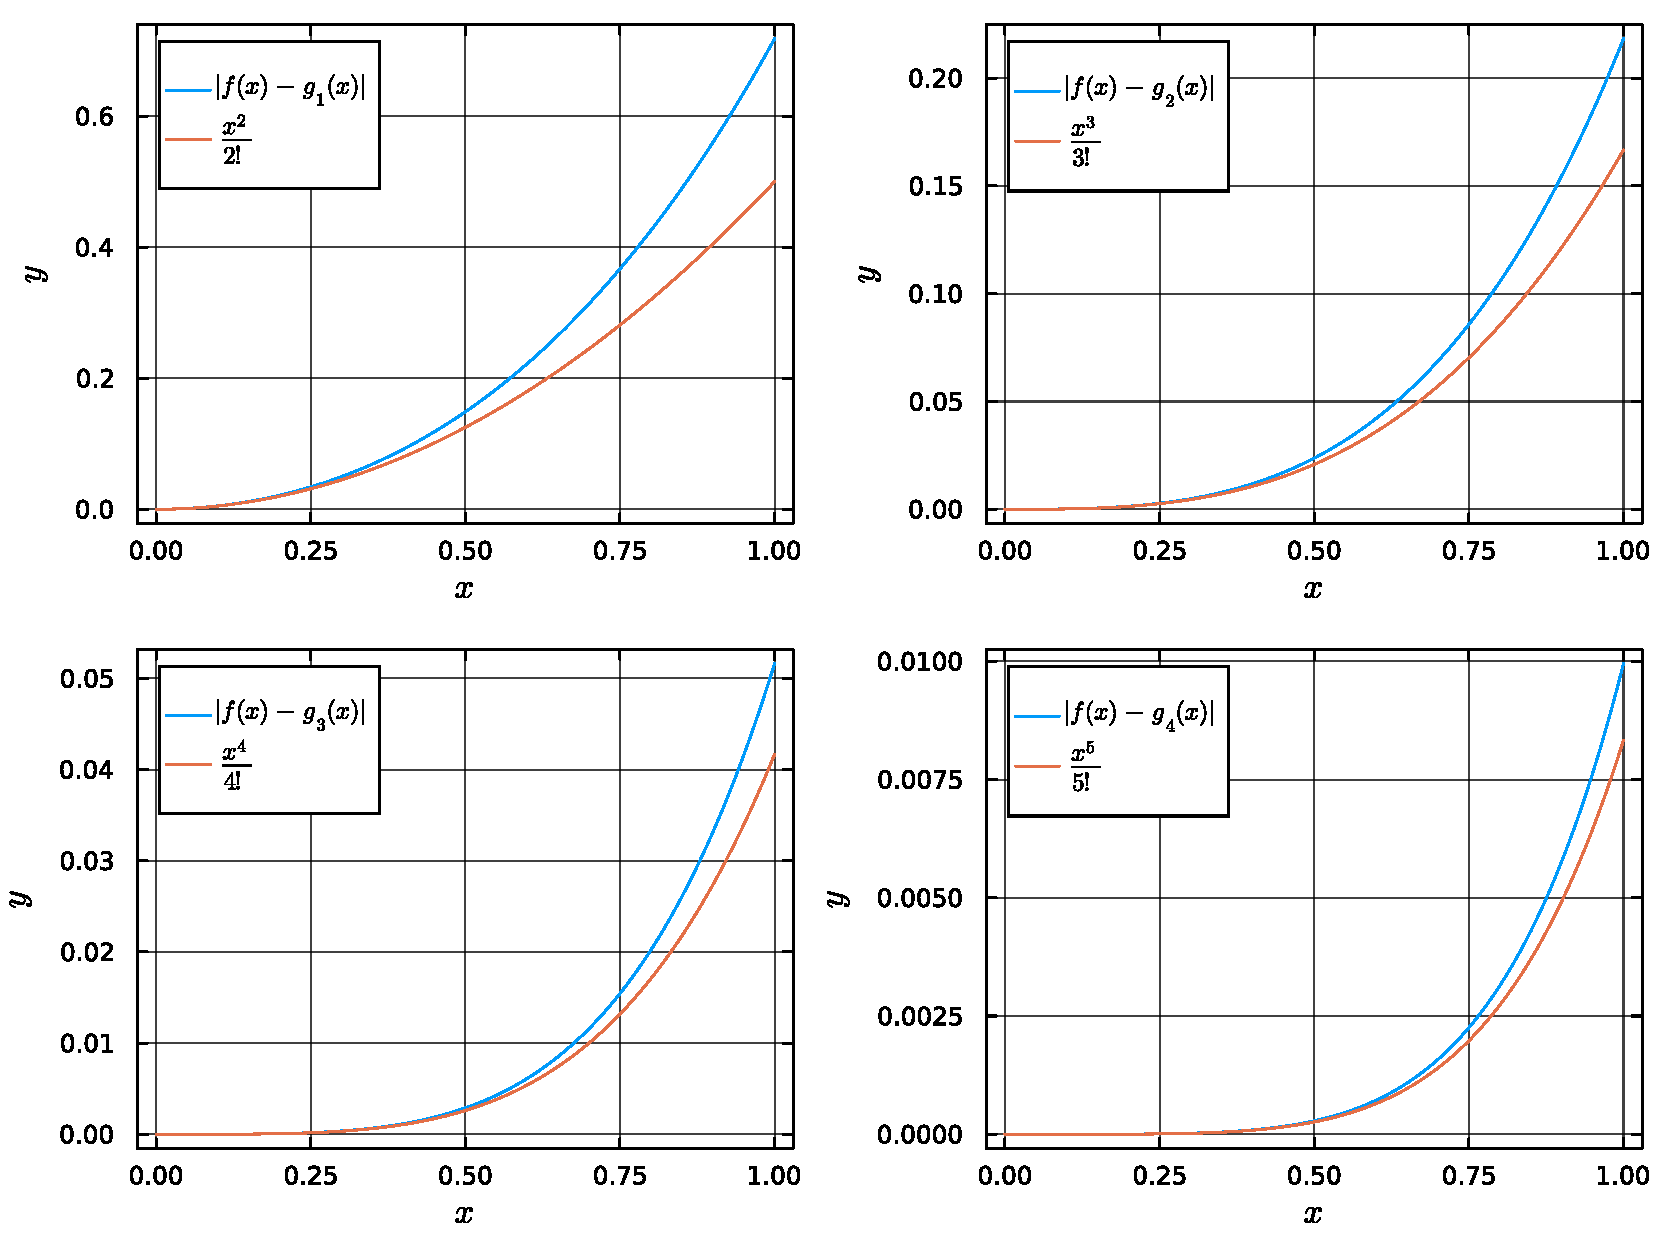
\includegraphics[width=0.8\textwidth]{1011.pdf}
    \caption{Confronto tra $\Delta$ e $\frac{x^{N+1}}{(N+1)!}$ per $N=1,2,3, 4$.}
    \label{fig:es1_0_1_1}
\end{figure}

La prima considerazione che possiamo fare è che all'aumentare di $N$ la funzione $\Delta$ 
assume valori sempre più vicini allo zero. Questo significa che la distanza tra il valore 
della funzione $f(x)$ presa in esame e la sua espansione di Taylor troncata all'ordine 
$N$ diminuisce. In effetti ci aspettiamo che la funzione $\Delta$ sia 
esattamente zero nel caso in cui $N \rightarrow \infty$. Inoltre possiamo notare che la funzione $\Delta$, in ognuno
dei grafici, è tanto più prossima allo zero quanto più ci si avvicina all'origine, poichè l'espansione in serie 
richiede $x \rightarrow 0$.\\
La seconda considerazione è che le funzioni $\Delta$ e $\frac{x^{N+1}}{(N+1)!}$ si 
avvicinano tra loro all'aumentare di $N$. Questo risponde alla richiesta dell'esercizio, 
cioè che l'errore scali come un polinomio di ordine $N+1$. 

\subsection{Esercizio 1.2.1}
Calcolare la seguente somma

$$
    \sum_{n=1}^\infty \frac{1}{n^2}=\frac{\pi^2}{6}
    =\lim_{N\to\infty} S(N)
    \quad
    \text{con}
    \quad
    S(N)=\sum_{n=1}^N \frac{1}{n^2}
$$

\begin{enumerate}
    \item Calcolare la somma in single precision utilizzando l'ordinamento normale,\\
    $n=1,2,3,\ldots,N$.
    \item Calcolare la somma in single precision utilizzando l'ordinamento inverso,\\
    $n=N,\ldots,2,1$.
    \item Studiare la convergenza di entrambe le implementazioni in funzione di $N$ tracciando il grafico di $|S(N)-\pi^2/6|$.
    \item Ripetere i punti da 1 a 3 utilizzando double precision.
    \item Sai spiegare cosa succede?
\end{enumerate}

\subsubsection{Soluzione}
Procediamo prendendo in esame i due casi, single precision e double precision.

\paragraph{Single precision:} 

Si riportano in figura \ref{fig:es1_2_1_1} gli errori di troncamento della serie 
$\sum_{n=1}^\infty \frac{1}{n^2}$, laddove $N$ è il troncamento. La somme sono state eseguite
con variabili di tipo Float32 (single precision).

\begin{figure}[ht!]
    \centering
    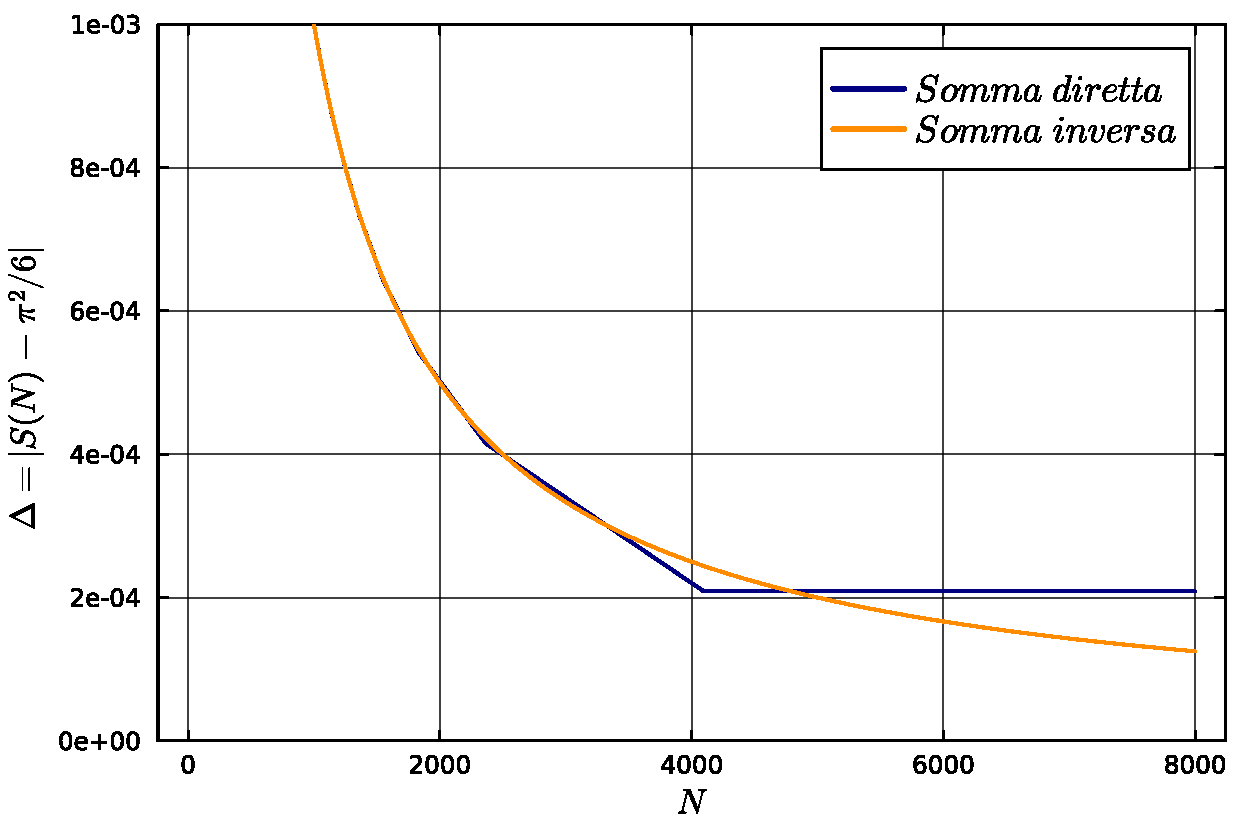
\includegraphics[width=0.8\textwidth]{1211.pdf}
    \caption{$S(N)=\sum_{n=1}^N \frac{1}{n^2}$ in single precision}
    \label{fig:es1_2_1_1}
\end{figure}

In figura \ref{fig:es1_2_1_1} notiamo due comportamenti degni di nota. Il primo riguarda
la curva blu, che arresta la sua discesa poco dopo $N = 4000$. 
Il secondo riguarda il discostarsi delle due curve, già a partire da 
$N \simeq 2000$, a causa dell'andamento a linea spezzata della curva blu.\\
La spiegazione del primo fenomeno è la seguente: nel caso della somma con ordinamento
diretto, all'aumento dell'indice di somma, gli addendi sono sempre più piccoli. In
particolare la somma comincia da 1, e sappiamo che dovrà raggiungere $\frac{\pi^2}{6} \simeq 1.64$ e perciò 
per tutto il processo la somma parziale resterà nell'intervallo $[1, 2)$. In tale intervallo la distanza tra due 
floating point numbers è $\epsilon_{mach} = 2^{-23}$. Osserviamo il grafico \ref{fig:es1_2_1_1}: la curva blu comincia ad essere 
costante a partire da $N = 4096 = 2^{12}$. Tale numero corrisponde all'addendo $\frac{1}{N^2} = 2^{-24}$, 
che è appena più piccolo di $\epsilon_{mach}$, ovvero della distanza tra due floating point numbers in $[1, 2)$, e quindi è
come sommare $0$. \\
La spiegazione del secondo fenomeno è simile: in questo caso alla somma viene aggiunto
un addendo che è più piccolo del precedente, ma non così tanto da essere più piccolo di $\epsilon_{mach}$. In
questo modo la somma viene migliorata, ma il nuovo addendo è arrotondato rispetto al suo valore vero. Il successivo
addendo, pur essendo differente in teoria, a causa dell'arrotondamento risulta essere uguale al precedente. Ciò fa
in modo che venga sommato sempre lo stesso numero, e così l'andamento della curva blu è lineare. \\
I due fenomeni non si verificano per la somma con ordinamento inverso perchè il primo numero ad essere sommato 
è molto piccolo. Questo fa in modo che i successivi floating point number siano molto vicini tra loro, è così sommare
l'addendo successivo fa cadere la somma parziale vicina al floating point number che la approssima. \\
\\
Si può mostrare matematicamente che gli errori $\Delta = |S(N)-\pi^2/6|$ scalano come $O(\frac{1}{N})$. Per verificare questa
affermazione possiamo interpolare la curva degli errori con un metodo che vedremo nella sezione \ref{sistemi_lineari}.
Sulla base delle considerazioni di questa sezione, possiamo aspettarci che sia più conveniente interpolare la curva 
con ordinamento inverso, perchè i valori che la compongono sono meno affetti da errori di tipo numerico. Utilizzando 
il modello linearizzato $log(\Delta) = -c*log(N)$ con $c = 1$ si ottiene per l'ordinamento inverso 
$c_{fit} = 1.00003$ e per quello diretto $c_{fit} = 0.986$. Come atteso il caso di ordinamento diretto restituisce un
risultato peggiore di quello inverso.


\paragraph{Double precision:}

Si riporta in figura \ref{fig:es1_2_1_2} un ingrandimento del grafico degli errori di troncamento della serie 
$\sum_{n=1}^\infty \frac{1}{n^2}$, laddove $N$ è il troncamento. La somme sono state eseguite
con variabili di tipo Float64 (double precision).

\begin{figure}[ht!]
    \centering
    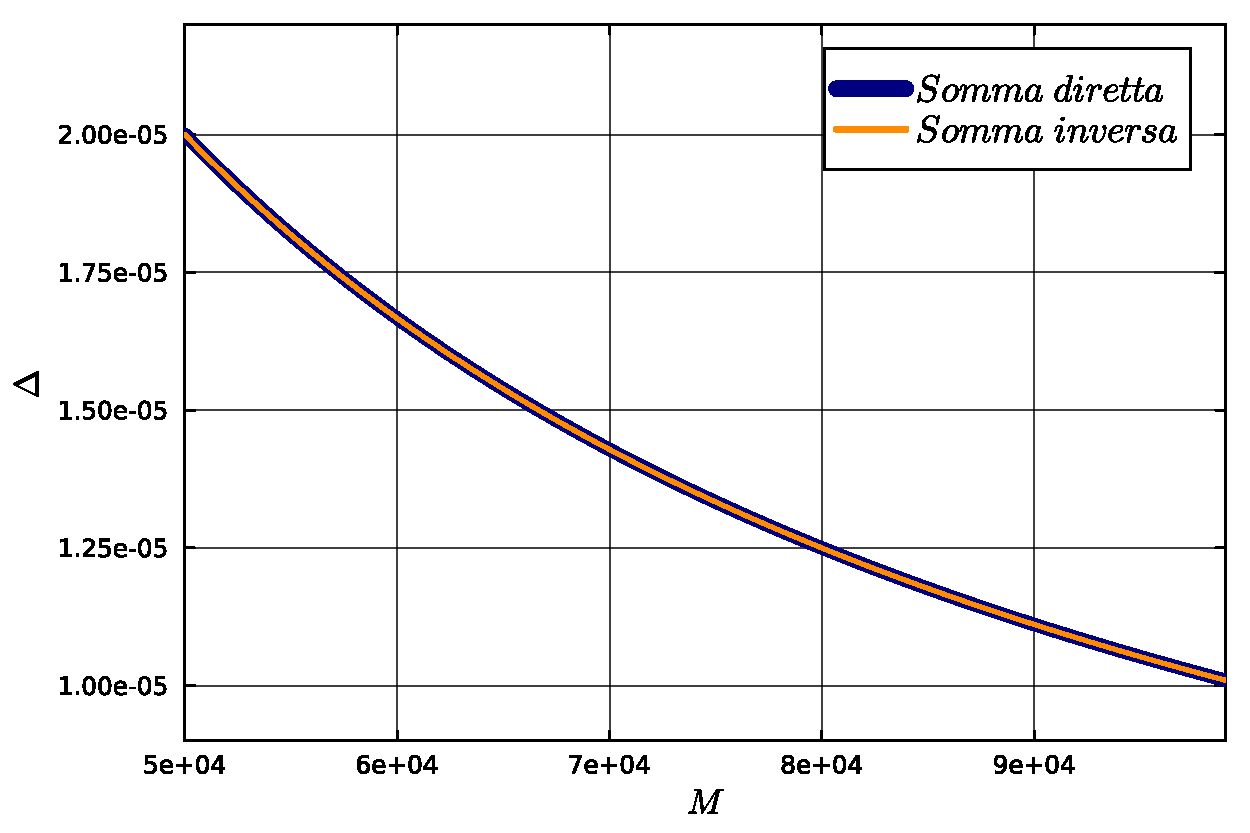
\includegraphics[width=0.8\textwidth]{1212.pdf}
    \caption{Ingrandimento di $S(N)=\sum_{n=1}^N \frac{1}{n^2}$ in double precision}
    \label{fig:es1_2_1_2}
\end{figure}

Nel caso di figura \ref{fig:es1_2_1_2} possiamo notare che le due curve sono sovrapposte, nonostante l'ingrandimento a 
valori di $N \in [5000, 10000]$. Per osservare un fenomeno simile a quello di 
figura \ref{fig:es1_2_1_1} dovremmo raggiungere valori di $N = 2^{26}$. Infatti l'approssimazione non migliora
quando vengono sommati numeri dell'ordine di $\epsilon_{mach}$ per double precision, cioè
 $\frac{1}{N^2} \simeq 2^{-52}$.

\subsection{Esercizio 1.4.1}

\section{Sistemi lineari}
\label{sistemi_lineari}
\subsection{Teoria}

\section{Radici di equazioni non lineari}
\subsection{Teoria}

\section{Interpolazioni}
\subsection{Teoria}

\section{Integrazione numerica}
\subsection{Teoria}

\section{Equazioni differenziali ordinarie}
\subsection{Teoria}

\end{document}